\documentclass{article}

\usepackage[math,lf,footnotefigures]{MyriadPro}
\renewcommand{\familydefault}{\sfdefault}

\usepackage{tikz}
\usetikzlibrary{arrows}
\usetikzlibrary{arrows.meta}
\usetikzlibrary{positioning}

\usepackage{xcolor}
\definecolor{ufzgray1}{RGB}{81,81,81}
\definecolor{ufzgray2}{RGB}{156,156,156}
\definecolor{ufzgray3}{RGB}{185,185,185}
\definecolor{ufzgray4}{RGB}{230,230,230}

\begin{document}
	
\pagestyle{empty}

\hspace*{-3cm}
	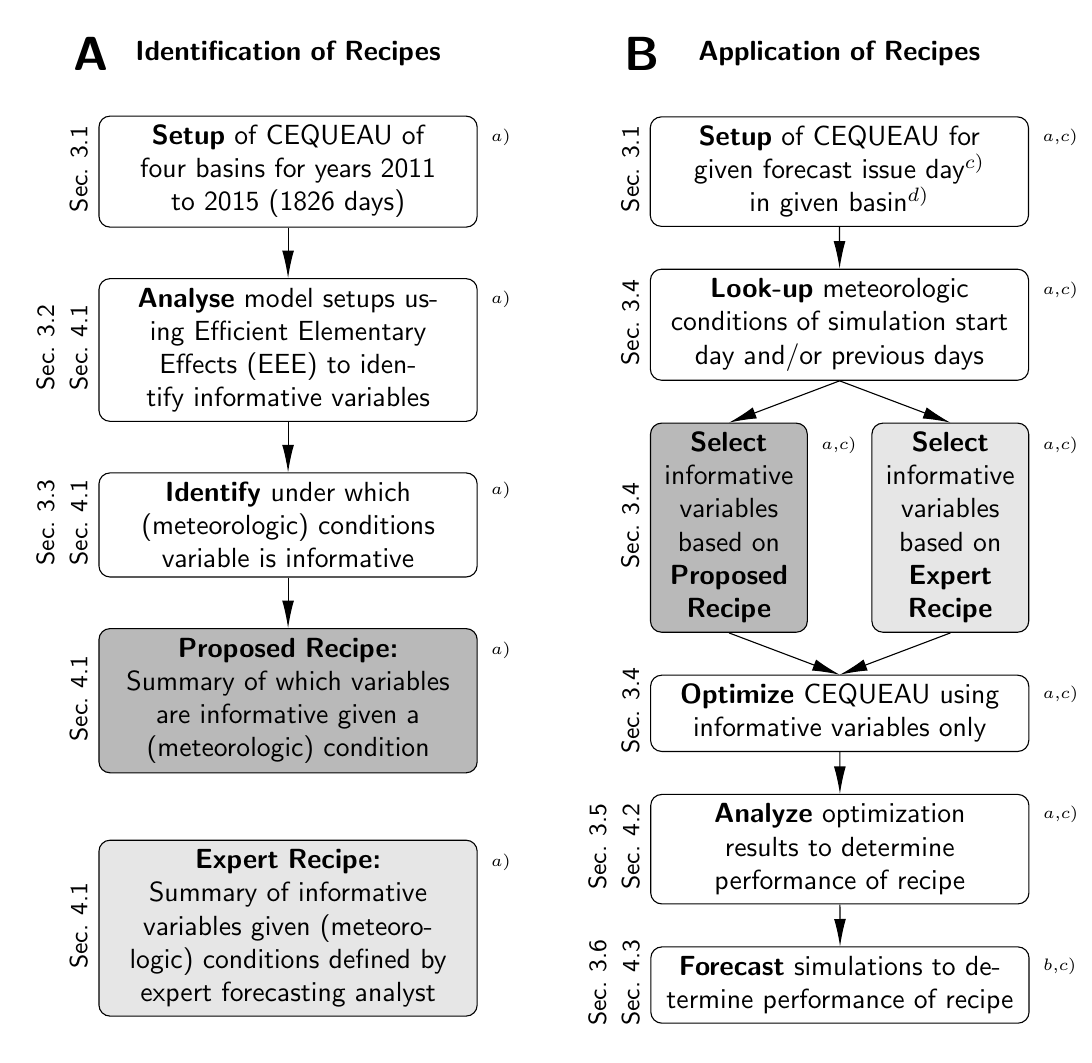
\begin{tikzpicture}[scale=2.5]
		\tikzstyle{block} = [rectangle, draw, fill=white!20, 
		text width=13em, text centered, rounded corners, minimum height=1em]
		\tikzstyle{noblock} = [rectangle, fill=white!20, 
		text width=14em, rounded corners, minimum height=1em]
		\tikzstyle{abcblock} = [rectangle, fill=white!20, 
		text width=1em, rounded corners, minimum height=1em]
		\tikzstyle{line} = [draw, -latex']
		\tikzstyle{line} = [draw,latex'-latex'new]
		
		% caption
		\node [noblock,align=center] (A) {\textbf{Identification of Recipes}};
		\node [noblock,align=center,right of=A,xshift=6cm] (B) {\textbf{Application of Recipes}};
		
		% ABC
		\node [abcblock,align=center,left of=A,xshift=-1.55cm] {{\LARGE \textbf{A}}};
		\node [abcblock,align=center,left of=B,xshift=-1.55cm] {{\LARGE \textbf{B}}};
		
		% Identification of Recipes
		\node [block, below of=A, node distance=1.5cm] (a1) {\textbf{Setup} of CEQUEAU of four basins for years 2011 to 2015 (1826 days)};
		\node [noblock,rotate=90,align=center,left=0.25cm of a1.west,text width=0.4em,xshift=-0.25cm] (a1sec) {\small Sec.~3.1};
		\node [noblock,rotate=0,align=left,right=0.05cm of a1.east,text width=0.4em,xshift=0.0cm,yshift=0.4cm] (a1note) {\small $^\text{a)}$};
		
		\node [block, below=0.64cm of a1.south, node distance=2.5cm] (a2) {\textbf{Analyse} model setups using Efficient Elementary Effects (EEE) to identify informative variables};
		\node [noblock,rotate=90,align=center,left=0.46cm of a2.west,text width=0.4em,xshift=-0.25cm] (a2sec) {\small Sec.~3.2\\Sec.~4.1};
		\node [noblock,rotate=0,align=left,right=0.05cm of a2.east,text width=0.4em,xshift=0.0cm,yshift=0.6cm] (a2note) {\small $^\text{a)}$};
		
		\node [block, below=0.64cm of a2.south, node distance=2.5cm] (a3) {\textbf{Identify} under which (meteorologic) conditions variable is informative};
		\node [noblock,rotate=90,align=center,left=0.46cm of a3.west,text width=0.4em,xshift=-0.25cm] (a2sec) {\small Sec.~3.3\\Sec.~4.1};
		\node [noblock,rotate=0,align=left,right=0.05cm of a3.east,text width=0.4em,xshift=0.0cm,yshift=0.4cm] (a3note) {\small $^\text{a)}$};
		
		\node [block, below=0.64cm of a3.south, node distance=2.5cm, fill=ufzgray3] (a4) {\textbf{Proposed Recipe:}\\ Summary of which variables are informative given a (meteorologic) condition};
		\node [noblock,rotate=90,align=center,left=0.25cm of a4.west,text width=0.4em,xshift=-0.25cm] (a2sec) {\small Sec.~4.1};
		\node [noblock,rotate=0,align=left,right=0.05cm of a4.east,text width=0.4em,xshift=0.0cm,yshift=0.6cm] (a4note) {\small $^\text{a)}$};
		
		\node [block, below=0.84cm of a4.south, node distance=2.5cm, fill=ufzgray4] (a5) {\textbf{Expert Recipe:}\\ Summary of informative variables given (meteorologic) conditions defined by expert forecasting analyst};
		\node [noblock,rotate=90,align=center,left=0.25cm of a5.west,text width=0.4em,xshift=-0.25cm] (a2sec) {\small Sec.~4.1};
		\node [noblock,rotate=0,align=left,right=0.05cm of a5.east,text width=0.4em,xshift=0.0cm,yshift=0.8cm] (a5note) {\small $^\text{a)}$};
		
		\node [block, below of=B, node distance=1.5cm] (b1) {\textbf{Setup} of CEQUEAU for\\ given forecast issue day$^\text{c)}$ \\ in given basin$^\text{d)}$};
		\node [noblock,rotate=90,align=center,left=0.25cm of b1.west,text width=0.4em,xshift=-0.25cm] (b2sec) {\small Sec.~3.1};
		\node [noblock,rotate=0,align=left,right=0.05cm of b1.east,text width=0.4em,xshift=0.0cm,yshift=0.4cm] (b1note) {\small $^\text{a,c)}$};
				
		\node [block, below=0.53cm of b1.south, node distance=2.5cm] (b2) {\textbf{Look-up} meteorologic conditions of simulation start day and/or previous days};
		\node [noblock,rotate=90,align=center,left=0.25cm of b2.west,text width=0.4em,xshift=-0.25cm] (b2sec) {\small Sec.~3.4};
		\node [noblock,rotate=0,align=left,right=0.05cm of b2.east,text width=0.4em,xshift=0.0cm,yshift=0.4cm] (b2note) {\small $^\text{a,c)}$};
		
		\node [block, below=0.53cm of b2.south, node distance=2.5cm, text width=5.0em, xshift=-4.0em, fill=ufzgray3] (b3a) {\textbf{Select} informative variables based on \textbf{Proposed Recipe}};
		\node [block, below=0.53cm of b2.south, node distance=2.5cm, text width=5.0em, xshift=4.0em, fill=ufzgray4] (b3b) {\textbf{Select} informative variables based on \textbf{Expert Recipe}};
		\node [noblock,rotate=90,align=center,left=0.25cm of b3a.west,text width=0.4em,xshift=-0.25cm] (b3sec) {\small Sec.~3.4};
		\node [noblock,rotate=0,align=left,right=0.05cm of b3a.east,text width=0.4em,xshift=0.0cm,yshift=1.0cm] (b3anote) {\small $^\text{a,c)}$};
		\node [noblock,rotate=0,align=left,right=0.05cm of b3b.east,text width=0.4em,xshift=0.0cm,yshift=1.0cm] (b3bnote) {\small $^\text{a,c)}$};
		
		\node [block, below=0.53cm of b3a.south, node distance=2.5cm, xshift=4.0em] (b4) {\textbf{Optimize} CEQUEAU using informative variables only};
		\node [noblock,rotate=90,align=center,left=0.25cm of b4.west,text width=0.4em,xshift=-0.25cm] (b4sec) {\small Sec.~3.4};
		\node [noblock,rotate=0,align=left,right=0.05cm of b4.east,text width=0.4em,xshift=0.0cm,yshift=0.2cm] (b4note) {\small $^\text{a,c)}$};
		
		\node [block, below=0.53cm of b4.south, node distance=2.5cm] (b5) {\textbf{Analyze} optimization results to determine performance of recipe};
		\node [noblock,rotate=90,align=center,left=0.46cm of b5.west,text width=0.4em,xshift=-0.25cm] (b5sec) {\small Sec.~3.5\\Sec.~4.2};
		\node [noblock,rotate=0,align=left,right=0.05cm of b5.east,text width=0.4em,xshift=0.0cm,yshift=0.4cm] (b5note) {\small $^\text{a,c)}$};
		
		\node [block, below=0.53cm of b5.south, node distance=2.5cm] (b6) {\textbf{Forecast} simulations to determine performance of recipe};
		\node [noblock,rotate=90,align=center,left=0.46cm of b6.west,text width=0.4em,xshift=-0.25cm] (b5sec) {\small Sec.~3.6\\Sec.~4.3};
		\node [noblock,rotate=0,align=left,right=0.05cm of b6.east,text width=0.4em,xshift=0.0cm,yshift=0.2cm] (b6note) {\small $^\text{b,c)}$};
		
		% lines A-B (realistic setup)
		\draw [-{Latex[length=3.5mm, width=1.5mm]}] (a1.south) -- (a2.north);
		\draw [-{Latex[length=3.5mm, width=1.5mm]}] (a2.south) -- (a3.north);
		\draw [-{Latex[length=3.5mm, width=1.5mm]}] (a3.south) -- (a4.north);
		
		\draw [-{Latex[length=3.5mm, width=1.5mm]}] (b1.south) -- (b2.north);
		\draw [-{Latex[length=3.5mm, width=1.5mm]}] (b2.south) -- (b3a.north);
		\draw [-{Latex[length=3.5mm, width=1.5mm]}] (b2.south) -- (b3b.north);
		\draw [-{Latex[length=3.5mm, width=1.5mm]}] (b3a.south) -- (b4.north);
		\draw [-{Latex[length=3.5mm, width=1.5mm]}] (b3b.south) -- (b4.north);
		\draw [-{Latex[length=3.5mm, width=1.5mm]}] (b4.south) -- (b5.north);
		\draw [-{Latex[length=3.5mm, width=1.5mm]}] (b5.south) -- (b6.north);
		
	\end{tikzpicture}
	
	
%	\hspace*{-3cm}
%	\begin{tikzpicture}[scale=2.5]
%	\tikzstyle{block} = [rectangle, draw, fill=white!20, 
%	text width=1em, text centered, rounded corners, minimum height=1em]
%	\tikzstyle{noblock} = [rectangle, fill=white!20, 
%	text width=12em, rounded corners, minimum height=1em]
%	\tikzstyle{line} = [draw, -latex']
%	
%	% process names
%	\node [noblock,align=left] (A) {Process 1\\ (e.g., infiltration)};
%	\node [noblock,align=left,below of=A] (B) {Process 2\\ (e.g., quickflow)};
%	\node [noblock,align=left,below of=B] (C) {Process 3\\ (e.g., evaporation)};
%	\node [noblock,align=left,below of=C] (D) {Process 4\\ (e.g., baseflow)};
%	\node [noblock,align=left,below of=D] (E) {Process 5\\ (e.g., snow balance)};
%	\node [noblock,align=left,below of=E] (F) {Process 6\\ (e.g., surf. runoff convol.)};
%	\node [noblock,align=left,below of=F] (G) {Process 7\\ (e.g., delay. runoff convol.)};
%	\node [noblock,align=left,below of=G] (H) {Process 8\\ (e.g., potential melt)};
%	\node [noblock,align=left,below of=H] (I) {Process 9\\ (e.g., percolation)};
%	\node [noblock,align=left,below of=I] (J) {Process 10\\ (e.g., remainder)};
%	%\node [noblock,align=left,below of=J] (K) {Process 11\\ (e.g., remainder)};
%	
%	% process options (simple setup)
%	\node [block, node distance=1.5cm,right of=A, xshift=0.7cm] (a1) {$A_1$};
%	\node [block, node distance=1.5cm,right of=a1] (a2) {$A_2$};
%	\node [block, node distance=1.5cm,right of=B] (b1) {$B_1$};
%	\node [block, node distance=1.5cm,right of=b1] (b2) {$B_2$};
%	\node [block, node distance=1.5cm,right of=b2] (b3) {$B_3$};
%	\node [block, node distance=1.5cm,right of=C, xshift=0.7cm] (c1) {$C_1$};
%	\node [block, node distance=1.5cm,right of=c1] (c2) {$C_2$};
%	
%	% process options (realistic setup)
%	\node [block, node distance=1.5cm,right of=a2, xshift=2.1cm] (d1) {$D_1$};
%	\node [block, node distance=1.5cm,right of=d1] (d2) {$D_2$};
%	\node [block, node distance=1.5cm,right of=b3, xshift=0.5cm] (e1) {$E_1$};
%	\node [block, node distance=1.5cm,right of=e1] (e2) {$E_2$};
%	\node [block, node distance=1.5cm,right of=e2] (e3) {$E_3$};
%	\node [block, node distance=1.5cm,right of=c2, xshift=2.1cm] (f1) {$F_1$};
%	\node [block, node distance=1.5cm,right of=f1] (f2) {$F_2$};
%	
%	% process options (Raven setup)
%	\node [block, node distance=1.5cm,right of=d2, xshift=1.2cm] (m1) {$M_1$};
%	\node [block, node distance=1.5cm,right of=m1] (m2) {$M_2$};
%	\node [block, node distance=1.5cm,right of=m2] (m3) {$M_3$};
%	\node [block, node distance=1.5cm,right of=e3, xshift=0.5cm] (n1) {$N_1$};
%	\node [block, node distance=1.5cm,right of=n1] (n2) {$N_2$};
%	\node [block, node distance=1.5cm,right of=n2] (n3) {$N_3$};
%	\node [block, node distance=1.5cm,right of=f2, xshift=2.0cm] (o1) {$O_1$};
%	\node [block, node distance=1.5cm,right of=o1] (o2) {$O_2$};
%	\node [block, node distance=1.5cm,right of=D, xshift=10.8cm] (p1) {$P_1$};
%	\node [block, node distance=1.5cm,right of=p1] (p2) {$P_2$};
%	\node [block, node distance=1.5cm,right of=E, xshift=10.0cm] (q1) {$Q_1$};
%	\node [block, node distance=1.5cm,right of=q1] (q2) {$Q_2$};
%	\node [block, node distance=1.5cm,right of=q2] (q3) {$Q_3$};
%	%\node [block, node distance=1.5cm,right of=q3] (q4) {$Q_4$};
%	\node [block, node distance=1.5cm,right of=F, xshift=11.5cm] (r1) {$R_1$};
%	\node [block, node distance=1.5cm,right of=G, xshift=11.5cm] (s1) {$S_1$};
%	\node [block, node distance=1.5cm,right of=H, xshift=11.5cm] (t1) {$T_1$};
%	\node [block, node distance=1.5cm,right of=I, xshift=11.5cm] (u1) {$U_1$};
%	\node [block, node distance=1.5cm,right of=J, xshift=11.5cm] (v1) {$V_1$};
%	%\node [block, node distance=1.5cm,right of=K, xshift=11.5cm] (w1) {$W_1$};
%	
%	% parameters (simple setup)
%	\node [align=left, right of=a1, xshift=-0.4cm] {\footnotesize $x_1$};
%	\node [align=left, right of=a2, xshift=-0.4cm] {\footnotesize $-$};
%	\node [align=left, right of=b1, xshift=-0.4cm] {\footnotesize $x_2$};
%	\node [align=left, right of=b2, xshift=-0.4cm] {\footnotesize $x_3$};
%	\node [align=left, right of=b3, xshift=-0.4cm] {\footnotesize $x_4$\\[-4pt]\footnotesize $x_5$};
%	\node [align=left, right of=c1, xshift=-0.4cm] {\footnotesize $x_6$};
%	\node [align=left, right of=c2, xshift=-0.4cm] {\footnotesize $x_7$};
%	
%	% parameters (realistic setup)
%	\node [align=left, right of=d1, xshift=-0.4cm] {\footnotesize $x_1$};
%	\node [align=left, right of=d2, xshift=-0.4cm] {\footnotesize $x_1$\\[-4pt]\footnotesize $x_2$};
%	\node [align=left, right of=e1, xshift=-0.4cm] {\footnotesize $x_2$};
%	\node [align=left, right of=e2, xshift=-0.4cm] {\footnotesize $x_3$};
%	\node [align=left, right of=e3, xshift=-0.4cm] {\footnotesize $x_4$\\[-4pt]\footnotesize $x_5$};
%	\node [align=left, right of=f1, xshift=-0.4cm] {\footnotesize $x_6$};
%	\node [align=left, right of=f2, xshift=-0.4cm] {\footnotesize $x_3$\\[-4pt]\footnotesize $x_7$};
%	
%	% parameters (Raven setup)
%	\node [align=left, right of=m1, xshift=-0.4cm] {\footnotesize $x_{1}$\\[-4pt]\footnotesize $x_{29}$};
%	\node [align=left, right of=m2, xshift=-0.4cm] {\footnotesize $x_{2}$\\[-4pt]\footnotesize $x_{29}$};
%	\node [align=left, right of=m3, xshift=-0.4cm] {\footnotesize $x_{3}$\\[-4pt]\footnotesize $x_{29}$};
%	\node [align=left, right of=n1, xshift=-0.4cm] {\footnotesize $x_{4}$\\[-4pt]\footnotesize $x_{29}$};
%	\node [align=left, right of=n2, xshift=-0.4cm] {\footnotesize $x_{5}$\\[-4pt]\footnotesize $x_{6}$\\[-4pt]\footnotesize $x_{29}$};
%	\node [align=left, right of=n3, xshift=-0.4cm] {\footnotesize $x_{5}$\\[-4pt]\footnotesize $x_{6}$\\[-4pt]\footnotesize $x_{7}$\\[-4pt]\footnotesize $x_{29}$};
%	\node [align=left, right of=o1, xshift=-0.4cm] {\footnotesize $x_{8}$\\[-4pt]\footnotesize $x_{29}$};
%	\node [align=left, right of=o2, xshift=-0.4cm] {\footnotesize $x_{8}$\\[-4pt]\footnotesize $x_{9}$\\[-4pt]\footnotesize $x_{10}$\\[-4pt]\footnotesize $x_{29}$};
%	\node [align=left, right of=p1, xshift=-0.4cm] {\footnotesize $x_{11}$};
%	\node [align=left, right of=p2, xshift=-0.4cm] {\footnotesize $x_{11}$\\[-4pt]\footnotesize $x_{12}$};
%	
%	\node [align=left, right of=q1, xshift=-0.4cm] {\footnotesize $x_{13}$\\[-8pt]\footnotesize $\ldots$\\[-6pt]\footnotesize $x_{18}$};
%	\node [align=left, right of=q2, xshift=-0.4cm] {\footnotesize $-$};
%	\node [align=left, right of=q3, xshift=-0.4cm] {\footnotesize $x_{18}$\\[-4pt]\footnotesize $x_{19}$};
%	%\node [align=left, right of=q4, xshift=-0.4cm] {\footnotesize $x_{18}$\\[-4pt]\footnotesize $x_{19}$\\[-4pt]\footnotesize $x_{20}$};
%	
%	\node [align=left, right of=r1, xshift=-0.4cm] {\footnotesize $x_{20}$\\[-4pt]\footnotesize $x_{21}$};
%	
%	\node [align=left, right of=s1, xshift=-0.4cm] {\footnotesize $x_{22}$\\[-4pt]\footnotesize $x_{23}$};
%	
%	\node [align=left, right of=t1, xshift=-0.4cm] {\footnotesize $x_{24}$\\[-8pt]\footnotesize $\ldots$\\[-6pt]\footnotesize $x_{27}$};
%	
%	\node [align=left, right of=u1, xshift=-0.4cm] {\footnotesize $x_{28}$\\[-4pt]\footnotesize $x_{29}$\\[-4pt]\footnotesize $x_{30}$};
%	
%	%\node [align=left, right of=v1, xshift=-0.4cm] {\footnotesize $x_{30}$\\[-4pt]\footnotesize $x_{31}$};
%	
%	\node [align=left, right of=v1, xshift=-0.4cm] {\footnotesize $-$};
%	
%	% lines A-B (simple setup)
%	\draw (a1.south) -- (b1.north);
%	\draw (a1.south) -- (b2.north);
%	\draw (a1.south) -- (b3.north);
%	\draw (a2.south) -- (b1.north);
%	\draw (a2.south) -- (b2.north);
%	\draw (a2.south) -- (b3.north);
%	
%	% lines B-C (simple setup)
%	\draw (b1.south) -- (c1.north);
%	\draw (b1.south) -- (c2.north);
%	\draw (b2.south) -- (c1.north);
%	\draw (b2.south) -- (c2.north);
%	\draw (b3.south) -- (c1.north);
%	\draw (b3.south) -- (c2.north);
%	
%	% lines A-B (realistic setup)
%	\draw (d1.south) -- (e1.north);
%	\draw (d1.south) -- (e2.north);
%	\draw (d1.south) -- (e3.north);
%	\draw (d2.south) -- (e1.north);
%	\draw (d2.south) -- (e2.north);
%	\draw (d2.south) -- (e3.north);
%	
%	% lines B-C (realistic setup)
%	\draw (e1.south) -- (f1.north);
%	\draw (e1.south) -- (f2.north);
%	\draw (e2.south) -- (f1.north);
%	\draw (e2.south) -- (f2.north);
%	\draw (e3.south) -- (f1.north);
%	\draw (e3.south) -- (f2.north);
%	
%	% lines M-N (Raven setup)
%	\draw (m1.south) -- (n1.north);
%	\draw (m1.south) -- (n2.north);
%	\draw (m1.south) -- (n3.north);
%	\draw (m2.south) -- (n1.north);
%	\draw (m2.south) -- (n2.north);
%	\draw (m2.south) -- (n3.north);
%	\draw (m3.south) -- (n1.north);
%	\draw (m3.south) -- (n2.north);
%	\draw (m3.south) -- (n3.north);
%	
%	% lines N-O (Raven setup)
%	\draw (n1.south) -- (o1.north);
%	\draw (n1.south) -- (o2.north);
%	\draw (n2.south) -- (o1.north);
%	\draw (n2.south) -- (o2.north);
%	\draw (n3.south) -- (o1.north);
%	\draw (n3.south) -- (o2.north);
%	
%	% lines O-P (Raven setup)
%	\draw (o1.south) -- (p1.north);
%	\draw (o1.south) -- (p2.north);
%	\draw (o2.south) -- (p1.north);
%	\draw (o2.south) -- (p2.north);
%	
%	% lines P-Q (Raven setup)
%	\draw (p1.south) -- (q1.north);
%	\draw (p1.south) -- (q2.north);
%	\draw (p1.south) -- (q3.north);
%	%\draw (p1.south) -- (q4.north);
%	\draw (p2.south) -- (q1.north);
%	\draw (p2.south) -- (q2.north);
%	\draw (p2.south) -- (q3.north);
%	%\draw (p2.south) -- (q4.north);
%	
%	% lines Q-R (Raven setup)
%	\draw (q1.south) -- (r1.north);
%	\draw (q2.south) -- (r1.north);
%	\draw (q3.south) -- (r1.north);
%	%\draw (q4.south) -- (r1.north);
%	
%	% lines R-S-T-U-V-W (Raven setup)
%	\draw (r1.south) -- (s1.north);
%	\draw (s1.south) -- (t1.north);
%	\draw (t1.south) -- (u1.north);
%	\draw (u1.south) -- (v1.north);
%	%\draw (v1.south) -- (w1.north);
%	
%	% caption
%	\node [noblock,align=center,above of=A,xshift=2.9cm,yshift=-0.3cm] {\textbf{Simple setup}};
%	\node [noblock,align=center,above of=A,xshift=8.0cm,yshift=-0.3cm] {\textbf{Realistic setup}};
%	\node [noblock,align=center,above of=A,xshift=13.0cm,yshift=-0.3cm] {\textbf{Raven setup}};
%	
%	\end{tikzpicture}

\end{document}



